% Packages --------------------------------------------------------------
\documentclass[10pt,a4paper]{article}
\usepackage[utf8]{inputenc}
\usepackage[english]{babel} % Added English as primary
\usepackage{url}
\usepackage[hidelinks]{hyperref}
\usepackage{amsmath, amsfonts, amssymb}
\usepackage{graphicx}
\usepackage{float}
\usepackage{lipsum}
\usepackage{multicol}
\usepackage{booktabs}
\usepackage{tabularx}
\usepackage{makecell}
\usepackage[table]{xcolor}
\usepackage{microtype} % Improves justification
\usepackage{newpxtext,newpxmath} % Elegant Palatino font
\usepackage{enumitem} % Better list control
\usepackage{fancyhdr} % Professional headers
\usepackage[left=2.00cm, right=2.00cm, top=2.50cm, bottom=2.00cm]{geometry}
\usepackage[most]{tcolorbox} % Per il riquadro dell'abstract
\usepackage{blkarray} % Pacchetto robusto per matrici con etichette
\usepackage{cuted}
\usepackage{caption}
\usepackage{array}
\usepackage{url}
\usepackage{eurosym}
\usepackage{wrapfig}
\captionsetup{
    labelfont=bf,      
    font=small,        
    format=plain,      % Allineamento pulito
    margin=20pt       
}
\setlength{\headheight}{20pt}
\addtolength{\topmargin}{-8pt}

% Color Definition ------------------------------------------------------
% Rosso Sapienza (Bordeaux)
\definecolor{sapienza}{RGB}{130, 36, 51}

% Annex box -------------------------------------------------------------
\usepackage[framemethod=TikZ]{mdframed}

% Define the style for your small annex box
\mdfdefinestyle{annexbox}{
    linecolor=gray,
    linewidth=0.5pt,
    roundcorner=2pt,
    backgroundcolor=gray!10,
    innertopmargin=5pt,
    innerbottommargin=5pt,
    innerleftmargin=10pt,
    innerrightmargin=10pt,
    userdefinedwidth=\textwidth, % Adjust width here
    align=center % Centers the box on the page
}
% Coloured Header  ------------------------------------------------------
\pagestyle{fancy}
\fancyhf{}
\fancyhead[L]{\small \textit{\textcolor{sapienza}{Industrial Symbiosis in Porto Marghera}}}
\fancyhead[R]{\small \textcolor{sapienza}{\thepage}}
\renewcommand{\headrule}{\hbox to\headwidth{\color{sapienza}\leaders\hrule height \headrulewidth\hfill}}

% Section Styling (Titoli delle sezioni)
\usepackage{titlesec}
\titleformat{\section}{\large\bfseries\color{sapienza}}{\thesection}{1em}{}

\begin{document}

% --- Header / Logo Section ---------------------------------------------
\noindent
\begin{minipage}[b]{0.25\textwidth}
    
\includegraphics[width=\textwidth]{sapienza.png}
\end{minipage}
\hfill
\begin{minipage}[b]{0.70\textwidth}
    \raggedleft
    \rmfamily 
    {\footnotesize \textsc{Sapienza Università di Roma} \\ 
    \textit{Department of Management Engineering} \\ 
    Academic Year 2025/2026}
\end{minipage}

\vspace{1pt}
\noindent\textcolor{sapienza}{\rule{\textwidth}{0.4pt}} % La linea sotto il logo

\vspace{4mm}

% --- Title Section -----------------------------------------------------
\begin{center}
    {\LARGE \textbf{Analysis of the Industrial Symbiosis in Porto Marghera \vspace{4pt}}} \\
    \vspace{4mm}
    {\large Bauzon C. A. $^{1}$, Ba D.$^{2}$, De Nardi A.$^{3}$, Socheleau H.$^{4}$}\\
    \vspace{3mm}
    \small $^1$\textit{1985325} \quad $^2$\textit{2244299} \quad $^3$\textit{2265252}\quad $^4$\textit{2230818}
\end{center}

\vspace{3mm}

% --- Abstract  --------------------------------------------------------
\begin{tcolorbox}[
    colback=sapienza!5,     % Sfondo bordeaux chiarissimo
    colframe=sapienza!20,   % Bordo bordeaux tenue
    arc=0mm,
    boxrule=0.5pt,
    left=15pt, right=15pt, top=10pt, bottom=10pt
]
    \small
    \textbf{\textcolor{sapienza}{Abstract ---}} This work analyzes part of the existing industrial symbiosis (IS) in Porto Marghera (VE). The analysis is carried out using the enterprise input-output approach modeling and assessing the economic and environmental benefit of the companies considered. Furthermore, the potential barriers of the system are examined and some solutions are provided. Finally, the work includes some possible policies that could be implemented to enhance the whole system. All data used in this work refer to the year 2019. 
    
\end{tcolorbox}

\vspace{3mm}

% ---- Beginning of body of text --------------------------------------- 
\begin{multicols}{2}
		\section{Introduction}
			\subsection{Ecodistretto di Porto Marghera description}
The Ecodistretto di Porto Marghera was born in 2017, after the interruption of the former waste-to-energy plant. Its creation was driven by two different companies, Ecoprogetto Venezia S.r.l. and Eco-Ricicli Veritas, which converged into one in 2022, thus becoming Eco+Eco S.r.l. . This company forms part of the Veritas group, a municipally owned S.p.A. and one of the largest multiutility in Italy. The former Ecoprogetto Venezia S.r.l. was an integrated facility for processing unsorted waste; meanwhile, Eco-Ricicli Veritas operated as a platform for sorting waste from separate collection. Now, the two plants are still divided, but together they provide an environmentally-safe management of waste for approximately 890.000 people (Gruppo Veritas, n.d.). The Ecodistretto also welcomes third-party companies engaged in recycling materials at the early stages of the value chain.

\subsection{Selected Companies}
 In this work, only three companies within Ecodistretto di Porto Marghera are considered, with the aim of making the modeling process easier, albeit without providing a full-size analysis of the area. The companies modeled in this work are: 
 \begin{enumerate}[leftmargin=*]
    \item \textbf{Veritas}: it works in the whole Province of Venice and in the municipality of Mogliano Veneto (TV). In this work, Veritas includes only the former Eco-ricicli Veritas, responsible for waste collection and separation, and Metalrecycling Venice, which instead receives metal waste and recycles it. Thus, in this work its only output is \textcolor{sapienza}{recycled metal}. 
    \item \textbf{Ecopatè}: it is a glass recycling plant located in Musile di Piave. Recently, the plant was bought by Sibelco S.p.A which has completely substituted Ecopatè. Its only output is \textcolor{sapienza}{recycled glass}. 
    \item \textbf{Rilegno}: it is the Italian national consortium responsible for the collection and recycling of wooden packaging. It was established in 1997 following the D. Lgs No. 22/1997 (Decreto Ronchi). Its only output is \textcolor{sapienza}{recycled wood products}. 
 \end{enumerate}

\begin{figure*}[t] 
    \centering
    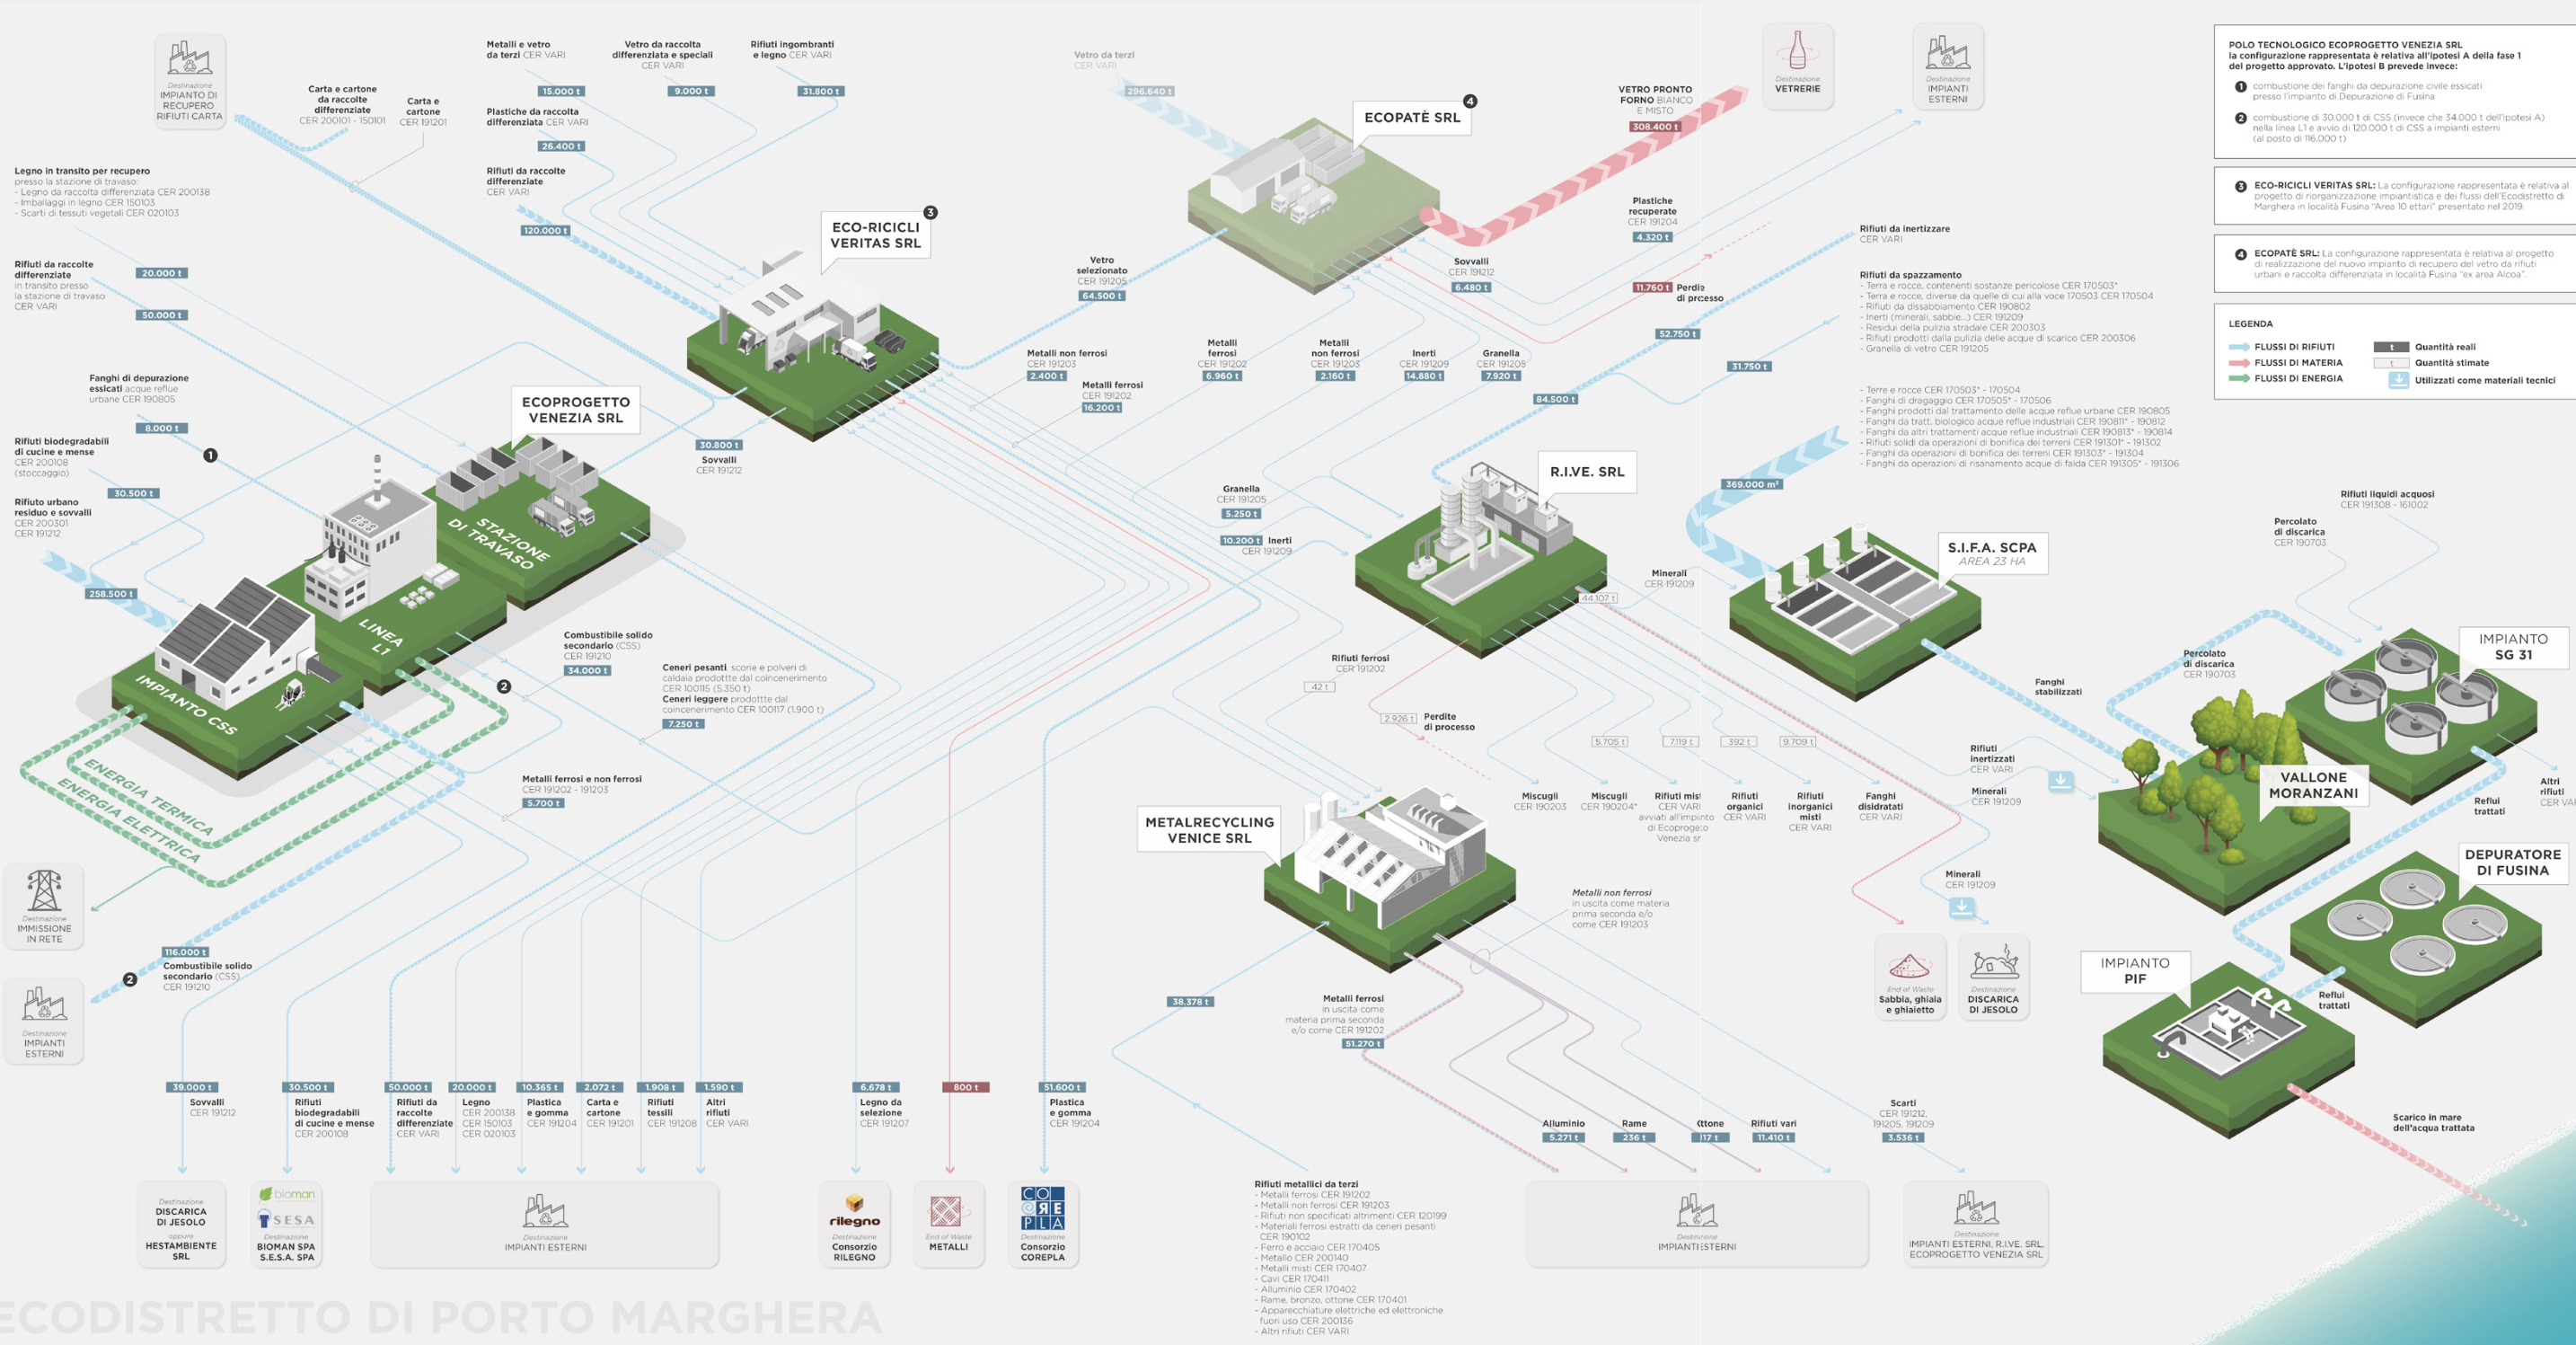
\includegraphics[width=\textwidth]{SchemaPM2.png}
    \caption{Visual representation of the whole industrial symbiosis in Porto Marghera. The image is taken by the 2019 report by Veritas and Comune di Venezia. (Veritas, 2019)}
    \label{fig:immagine_larga}
\end{figure*}	
		\section{IS Type}
           Industrial symbiosis manifests in a wide variety of forms. The most common way to classify IS is according to the user and the use-purpose of the exchanged good. This is summarized in a clear way into a table 1: 
           \begin{table}[H]
            \centering
            \small
            \begin{tabularx}{\linewidth}{>{\raggedright\arraybackslash}p{1.8cm} X X}
             \toprule
        & \textbf{Input replacement} & \textbf{Product development} \\
        \midrule
        \textbf{Internal use} & A company uses its own waste / product to replace an input & A company uses its waste to develop a new product \\
        \addlinespace[10pt]
        \textbf{External use} & \cellcolor{red!15} A different company uses the waste to replace an input & A different company uses the waste to develop a new product \\
        \bottomrule
            \end{tabularx}
             \caption{The four types of IS}
            \end{table}
\noindent Ecodistretto di Porto Marghera falls under the External use - Input replacement type of industrial symbiosis. Here, no companies develop a new product due to the implementation of IS. Additionally, the waste needs to be treated to be reused, so it a case of \textcolor{sapienza}{\textbf{imperfect IS}}.
		\section{Enterprise Input-Output approach modeling}
            % --------- Body text  --------
\subsection{Data}
The modeling of the selected IS was carried out using a part of the data presented in Figure \ref{fig:immagine_larga}. Since not all of the fluxes of the sheet were included, in this subsection an explanation of the used data is provided. \\

\noindent Firstly, in \textbf{Veritas} (which integrates Ecoprogetto-Ricicli and MetalRecycling Venice), the incoming waste streams are chosen according to the final output of the three companies (see section 1.2). This means that only metal waste, glass waste, wood waste and mixed waste are included because the three companies produce only wood packaging, glass, and metal. This choice was made because considering other types of waste (such as plastic) would misrepresent the environmental benefit of the whole IS assessed later in the work. The waste is considered to be coming from the province of Venice and the municipality of Mogliano Veneto (TV), consequently from a community of approximately 890.000 people (Gruppo Veritas, n.d.).
Turning to Veritas's outgoing waste, two streams are recovered by being sent to the other two companies, meanwhile only the mixed waste coming out from MetalRecycling Venice was considered as <<waste to landfill>> 
\begin{equation*}
    w_{\text{Veritas,mix}}=\underset{\text{mixed waste}}{11410t} + \underset{\text{scraps}}{3536t} = 14946t
\end{equation*}
Secondly, in \textbf{Rilegno} the incoming waste is only wood, which comes in through two different flows: one from Veritas and another from other parts of Italy. The amount of wood given to Rilegno by the other regions in Italy was taken by the Annual Balance of Rilegno of 2019, and the amount of the incoming wood waste to Veritas was subtracted from that number. In 2019, Rilegno was able to recycle 63,8 \% of the recovered wood (Rilegno, 2019, p.36), which means that 36,2 \% went to landfill.
\begin{equation*}
    w_{\text{Rilegno,wood}}=x_{\text{Rilegno}}*36,2\%
\end{equation*}
Finally, in \textbf{Ecopatè} the only incoming waste is the selected glass provided by Veritas. This is the only company of the model that has an external input, which is still glass but coming from third parts.
Ecopatè's waste to landfill is considered as the sum of the glass scraps and other inerts given to R.I.V.E. S.r.l. which processes them to go to the landfill (see Figure \ref{fig:immagine_larga} for reference). Ecopatè also has some metal waste as a result of the glass treatment that is given back to Veritas to be recycled.
\begin{equation*}
    w_{\text{Ecopatè,glass}}=\underset{\text{inerts}}{14880 t} + \underset{\text{glass scraps}}{7290t}= 22800t 
\end{equation*}
\begin{equation*}
    w_{\text{Ecopatè,metal}}=\underset{\text{nonferrous metals}}{2160t}+\underset{\text{ferrous metals}}{6960t}=9120t
\end{equation*}
\vspace{3mm}

\noindent Table \ref{tab:wastetable} provides a representation of the waste distribution: in D the chosen fluxes coming from the 890.000 community are listed and in E the amount of wood waste coming from other parts of Italy is presented.
% ----- Table ----------
\begin{table*}[t]
\centering
\begin{tcolorbox}[
    colback=sapienza!5,     % Sfondo bordeaux chiarissimo
    colframe=sapienza!20,   % Bordo bordeaux tenue
    arc=3pt,                 % Smussatura degli angoli
    boxrule=1pt,             % Spessore del bordo
    width=\textwidth,        % Larghezza del box
    halign=center            % Centra il contenuto nel box
]
    \begin{tabular}{c | c c c c c | c}
    \toprule
    \textbf{Waste type} & \textbf{A} & \textbf{B} & \textbf{C} & \textbf{D} & \textbf{E} & \textbf{Total} \\
    \midrule \midrule 
    $w_{wood}$ & 0 & 0 & 1245353 t & 31800 t & 3408402 t  & 4685555 t \\
    \midrule
    $w_{glass}$ & 0 & 22800 t & 0 & 9000 t & 0 & 31800 t \\
    \midrule
    $w_{metal}$ & 0 & 9120 t & 0 & 44078 t  & 0 & 53198 t \\
    \midrule
    $w_{mix}$ & 14946 t & 0 & 0 & 135000 t & 0 & 149946 t \\
    \bottomrule
    \end{tabular}
\end{tcolorbox}

\vspace{5pt}
\caption{Tabular representation of the calculation of the waste vector}
\label{tab:wastetable}
\end{table*}
\newpage
\subsection{The Black Box method}
In figure \ref{fig:scheme}, the whole system is represented using the black box method, which treats each company as an entity that processes what comes in to get a product (output). The process always involves the production of some waste. The different flows are represented using arrows of specific colors, as explained in the legend. Each box is named by a letter displayed on the upper right side of the box, in order to show clearly the computation of the matrixes in the following part. 
\begin{center}
    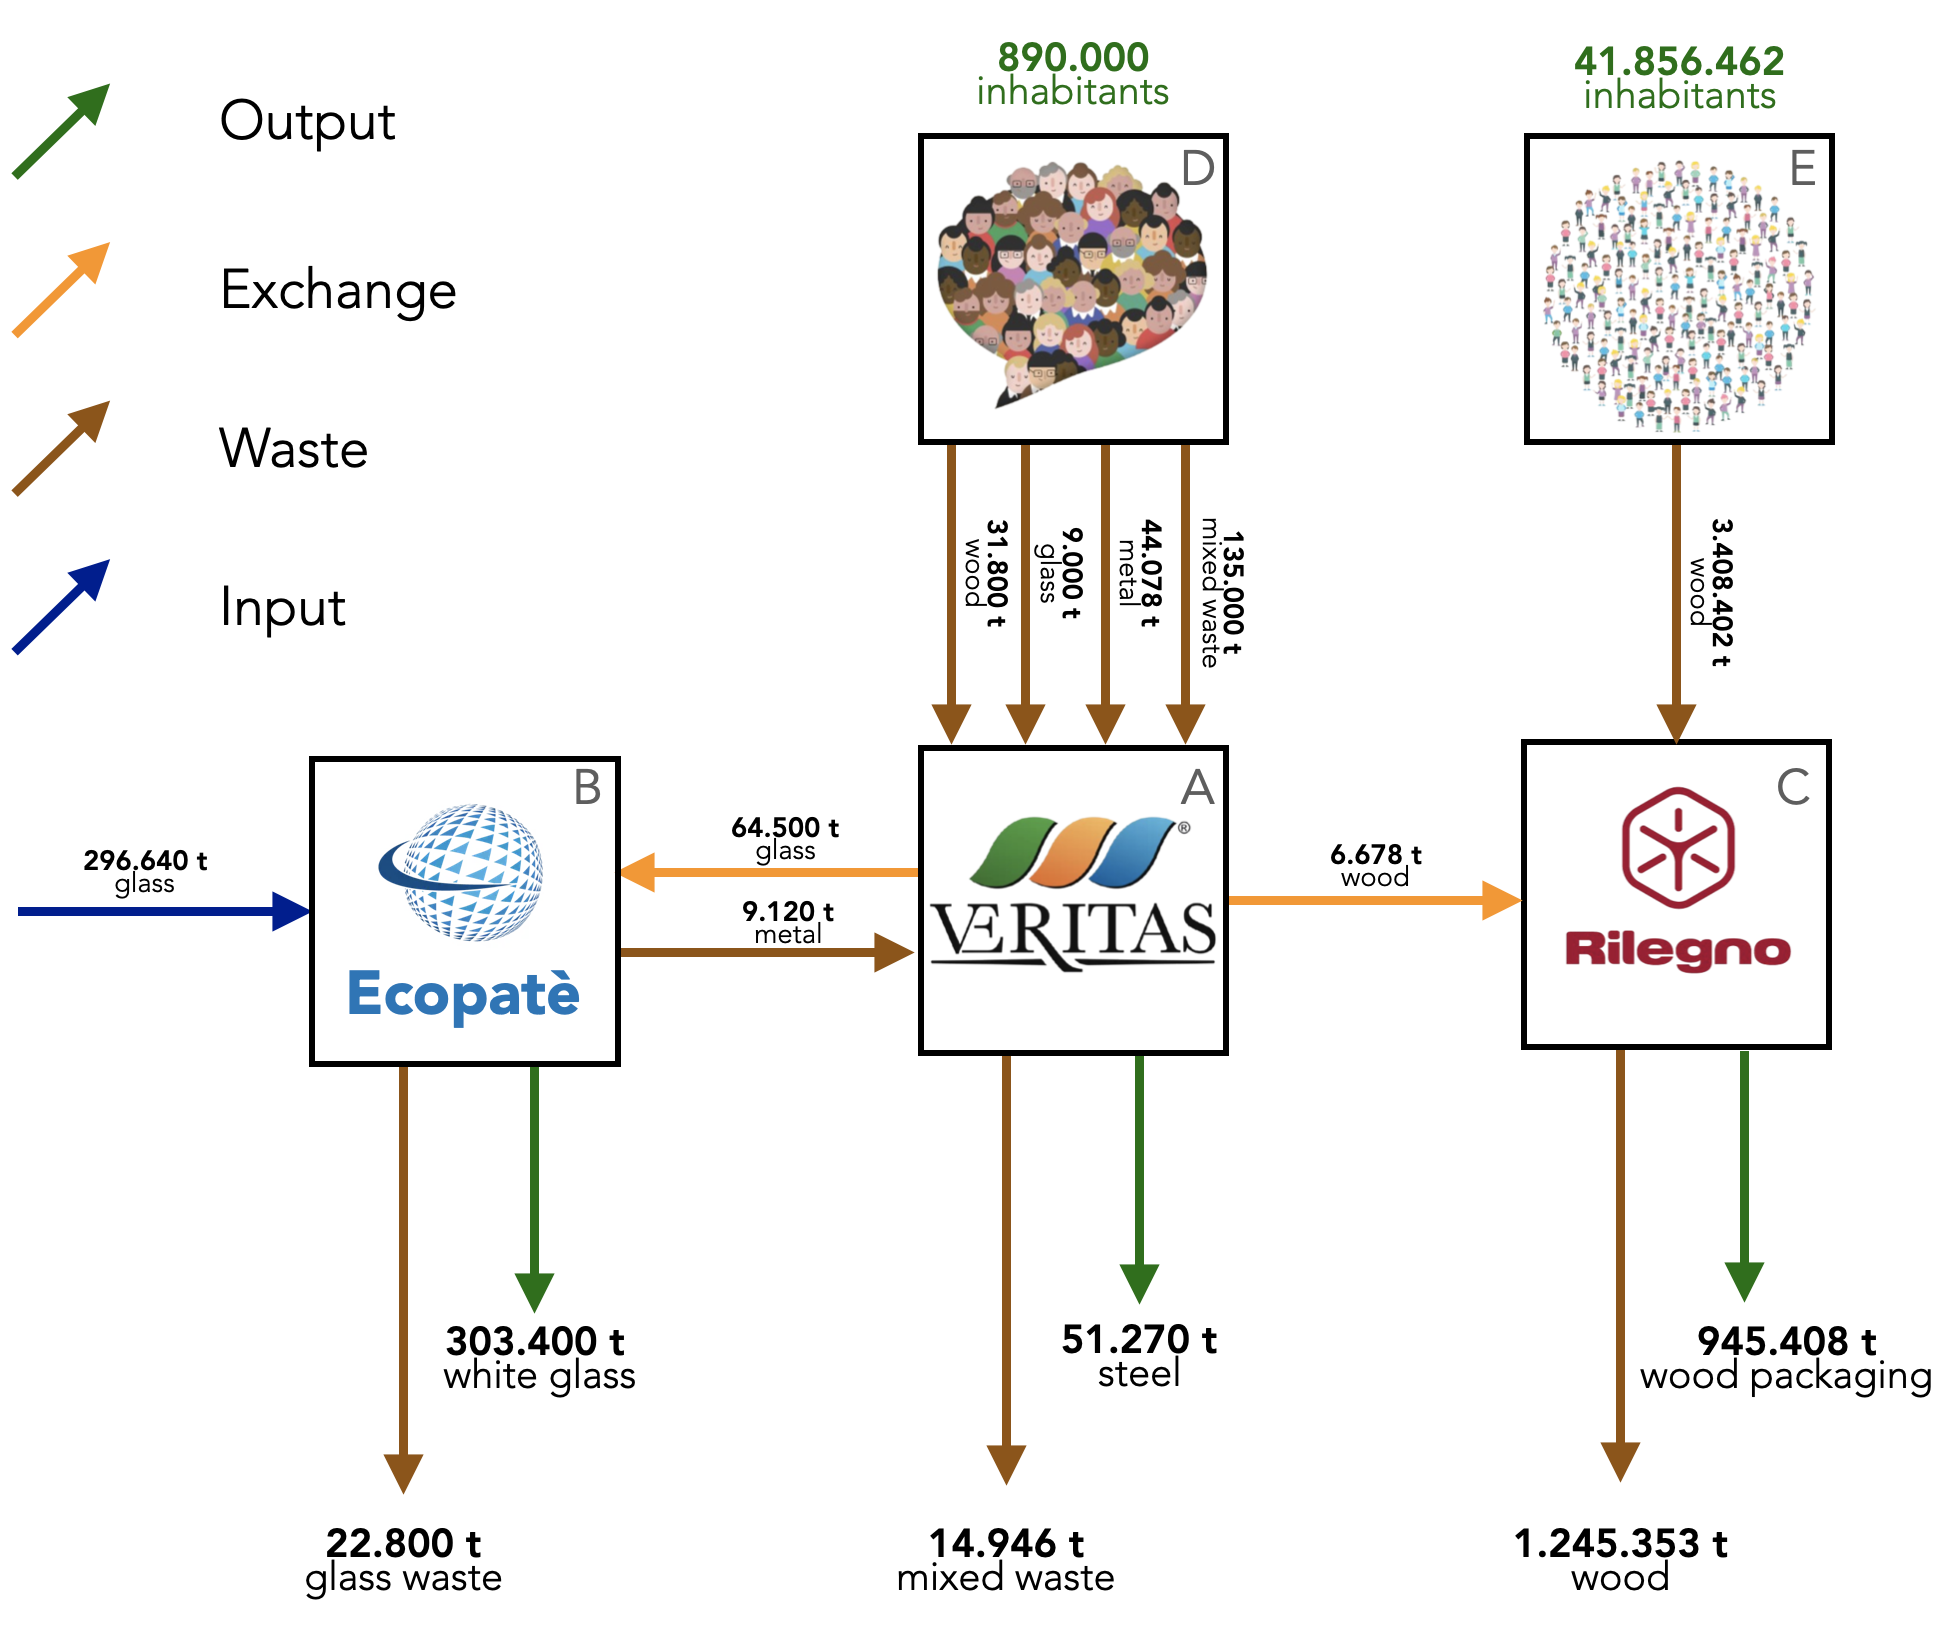
\includegraphics[width=0.95\linewidth]{schemapm.png}
    \captionof{figure}{Representation of the model through the black boxes method. Image created by the authors.}
    \label{fig:scheme}
\end{center}
As shown in figure \ref{fig:scheme}, to accurately map the IS, two additional boxes were included to represent the sources of waste and wood provided to Veritas and Rilegno, respectively. The group D represents the inhabitants of the Province of Venice and the municipality of Mogliano Veneto (TV) (Gruppo Veritas, n.d.) whereas group E considers the number of people that are served by Rilegno (Rilegno, 2019, p.14). 

%--input vector
\subsection{Vectors and Matrixes}
\subsubsection{Input vector}
The input vector shows the only present input of the system, that is the glass externally purchased by Ecopatè. Consequently, it is a vector with just one element.
        \begin{equation}
          \vec{r}=  
         \begin{bmatrix}
            r_{glass}
         \end{bmatrix}=
         \begin{bmatrix}
            296670
         \end{bmatrix}
        \end{equation}
        
 %--output vector
 \subsubsection{Output Vector}
 The output vector of the Ecodistretto di Porto Marghera considers the final outputs of each black box of the system. It is important to note that the output for boxes D and E is the number of inhabitants served by the respective company (Gruppo Veritas, n.d.) (Rilegno, 2019, p.14).
        \begin{equation}
            \vec{x}=
            \begin{bmatrix}
                x_{\text{Veritas}}\\
                x_{\text{Ecopatè}}\\
                x_{\text{Rilegno}}\\
                x_{\text{C.Veritas}}\\
                x_{\text{C.Rilegno}}\\
            \end{bmatrix}
            =
            \begin{bmatrix}
                51270 \\
                303400 \\
                945408 \\
                890000 \\
                41856462 \\
            \end{bmatrix}
        \end{equation}

%--waste vector
\subsubsection{Waste vector}
The waste vector regroups the different types of waste that appear in the system. Each element of the vector is the sum of all the specific waste that appears in the system. For more information on how the calculation is carried out, see Table \ref{tab:wastetable}.
        \begin{equation}
            \vec{w}=
            \begin{bmatrix}
                w_{wood} \\
                w_{glass} \\
                w_{metal} \\
                w_{mix}
            \end{bmatrix}
            =
            \begin{bmatrix}
                4685555 \\
                31800 \\
                53198 \\
                149946 
            \end{bmatrix}
        \end{equation}

 %-- Input matrix
 \subsubsection{Input matrix}
 The input matrix shows the distribution of each input among the different companies. In this case, the fact that there is only one input in the entire system implies that the matrix has only one row. Furthermore, each element of the matrix is calculated by dividing the input of the considered enterprise by its own output. The formula for each element of the matrix is the following one: 
 \begin{equation}
     r_{glass,j}=\frac{r_{glass}}{x_j}
 \end{equation}
 which leads to the input matrix for this case: 
 \begin{equation}
     R=
     \begin{bmatrix}
         0 & 0,98 & 0 & 0 & 0
     \end{bmatrix}
 \end{equation}
 
 %-- Waste matrix
 \subsubsection{Waste matrix}
  The waste matrix represents the distribution of each type of waste among the different companies of the model. Each element of the matrix is obtained using the formula (6):
 \begin{equation}
     w_{ij}=\frac{w_i}{x_j} \\
 \end{equation}
 where $w_i$ is the type of waste (wood, glass, etc.) and $x_j$ is the considered company (Veritas, ..., C.Rilegno).
\begin{equation}
    \label{eq:matrice_rifiuti}
    W = 
        \begin{blockarray}{cccccc}
        % Intestazioni di colonna
         & \text{A} & \text{B} & \text{C} & \text{D} & \text{E} \\
        \begin{block}{l[ccccc]}
        % Righe con etichetta laterale e contenuto
    w_{\text{wood}}  & 0    & 0 & 1,32 & 0,4  & 0,08 \\
    w_{\text{glass}} & 0    & 0 & 0    & 0,01 & 0    \\
    w_{\text{metal}} & 0    & 0 & 0    & 0    & 0    \\
    w_{\text{mix}}   & 0,29 & 0 & 0    & 0,15 & 0    \\
         \end{block}
         \end{blockarray}
\end{equation}

 %-- Z matrix
 \subsubsection{Z matrix}
 Finally, the Z matrix quantifies the exchanges between companies in tons. It specifies the participants and the amounts exchanged, reflecting only the two transactions depicted in Figure \ref{fig:scheme}.
 \begin{equation}
    \label{eq:matrice_z}
    Z = 
        \begin{blockarray}{cccccc}
        % Intestazioni di colonna
         & \text{A} & \text{B} & \text{C} & \text{D} & \text{E} \\
        \begin{block}{l[ccccc]}
        % Righe con etichetta laterale e contenuto
    A  & 0    & 64500 & 6678 & 0  & 0 \\
    B  & 0    & 0      & 0     & 0  & 0 \\
    C  & 0    & 0      & 0     & 0  & 0 \\
    D  & 0    & 0      & 0     & 0  & 0 \\
    E  & 0    & 0      & 0     & 0  & 0 \\
         \end{block}
         \end{blockarray}
\end{equation}
\end{multicols}
        \section{IS benefits}
            \subsection{Economic benefit}
\begin{multicols}{2}
\noindent The economic benefit (EB) is calculated using formula (9) which estimates how much each company can save by implementing industrial symbiosis.
\begin{equation}
    EB = [(dc+pc)-(rc+tc)]
\end{equation}
where 
\begin{itemize}[nosep]
    \item $dc =$ waste disposal cost
    \item $pc =$ input purchase cost
    \item $rc =$ treatment cost
    \item $tc =$ transportation cost
\end{itemize}
\noindent As a matter of fact, the input purchase cost and the waste disposal cost are two expenses present when IS does not exist. These expenses are reduced or completely avoided when IS is implemented because the input is substituted by the waste of another company. However, with industrial symbiosis, the external waste usually needs to be treated and transported, therefore there are two additional costs. Therefore, IS is convenient and gives an economic benefit to the company as long as the $rc$ and $tc$ are lower than the sum of $dc$ and $pc$. In other words, $EB>0$ must be valid. \\
In the analyzed system, the disposal cost for general mixed waste in Italy is \EUR{55}/ton (European Commission, 2022). This value is considered valid for the three selected companies. \\
\end{multicols}

\newtcolorbox{companybox}[1]{
    colback=sapienza!5,
    colframe=sapienza!20,
    arc=2mm,
    boxrule=0.8pt,
    left=4mm, right=4mm, top=3mm, bottom=3mm,
    title=\textbf{#1},
    coltitle=black,
    fonttitle=\large,
    attach title to upper=\quad,
    after skip=1.5em
}

\begin{companybox}{Veritas}
Veritas is a waste collection company, therefore, it does not have an input purchase cost. In contrast, it does have a transportation and treatment cost, which is extracted from their annual financial statement. In 2019, Metalrecycling Venice (the only part of Veritas that treats metal) spent \EUR{370.344} on transportation, \EUR{29527} on electricity and \EUR{5.635} on water (Metalrecycling Venice, 2020). Metal is usually treated in an electric arc furnace and is cooled with water. Thus, the treatment cost is considered as the sum of the cost of water and electricity. These amounts are divided by the total annual output to get the cost in \euro / ton.

\vspace{2mm}
\centering
\begin{tabular}{c|c|c|c|c}
    $dc$ & $pc$ & $rc$ & $tc$ & \textbf{Total} \\ \hline
    \EUR{55}/t & 0 & \EUR{0.6}/t & \EUR{6,5}/t & \textbf{\EUR{47,9}/t}
\end{tabular}
\end{companybox}
\vspace{2mm}

\begin{companybox}{Rilegno}
Rilegno is a national consortium that was created to recycle wood products. For this reason, it does not have an input purchase cost, as stated for Veritas. In contrast, it has a transportation and treatment cost, which is declared in the annual financial statement. In 2019, Rilegno spent \EUR{730.759} + \EUR{450.433} on treatment and \EUR{11.736.842} + \EUR{15.656.500} on transportation (Rilegno, 2020).

\vspace{2mm}
\centering
\begin{tabular}{c|c|c|c|c}
    $dc$ & $pc$ & $rc$ & $tc$ & \textbf{Total} \\ \hline
    \EUR{55}/t & 0 & \EUR{1,25}/t & \EUR{29}/t & \textbf{\EUR{24,75}/t}
\end{tabular}
\end{companybox}

\vspace{2mm}

\begin{companybox}{Ecopatè}
 Ecopatè is the only plant among the selected three that would have an input purchase cost. In 2019, recycled glass cost \EUR{71}/t (Eurostat, 2022). Concerning the treatment cost, the Italian national consortium for glass recycling CoReVe states that in 2019 \EUR{82.783.086}  was spent to produce 2.069.407 tons of recycled glass (CoReVe, 2020, Bilancio d'esercizio)(CoReVe, 2020, Risultati). Therefore, in 2019 the treatment cost of glass was \EUR{40}/t. This amount is considered as the mean cost of glass treatment, also valid for Ecopatè. Finally, the transportation cost was calculated considering the type of truck used to take glass from Veritas to Ecopaté (see Note 1).
 
\vspace{2mm}
\centering
\begin{tabular}{c|c|c|c|c}
    $dc$ & $pc$ & $rc$ & $tc$ & \textbf{Total} \\ \hline
    \EUR{55}/t & \EUR{71}/t & \EUR{40}/t & \EUR{3,5}/t & \textbf{\EUR{82,5}/t}
\end{tabular}
\end{companybox}

\noindent In conclusion, all economic benefits are positive, as it should be for the industrial symbiosis to be convenient for each company. 
\vspace{2mm}
\begin{mdframed}[style=annexbox]
    \small \textbf{Note 1:} The truck used by Veritas to deliver waste is Iveco EuroCargo that uses 18,5 liters of gasoline per 100 km (Lavori Pubblici, 2015). The distance between Ecopatè plant and Veritas plant is a bit less than 100 km (sum of back and forth), and the price of gasoline in 2019 in northern Italy was 1,4 €/l (FIGISC, 2019). EuroCargo weight when completely full 12 t and when empty 4,5 t, that means it can carry approximately 7,5 tons. That leads to 3,5 €/t over 100 km
\end{mdframed}
% -----------------------------------------------------
\subsection{Environmental benefit}
The environmental benefit is defined here as the difference in the percentage of waste sent to landfills with and without industrial symbiosis. To evaluate the percentage of waste to landfill with IS, the calculation considers the actual waste over the output of the selected company: 
\begin{equation}
   \underset{\text{with IS}}{\text{env. b.}} = \frac{\text{waste to landfill with IS}}{\text{output}}
\end{equation}
Instead, to assess the environmental benefit without IS, the waste at the numerator considers how much waste would go to landfill if companies did not cooperate: 
\begin{equation}
    \underset{\text{without IS}}{\text{env. b.}} = \frac{\text{waste to landfill without IS}}{\text{output}}
\end{equation}
Therefore, the difference between (11) and (10) is the actual environmental benefit:
\begin{equation}
    \text{env.b.} = \underset{\text{without IS}}{\text{env.b.}} - \underset{\text{with IS}}{\text{env.b.}} 
\end{equation}
For \textbf{Veritas}, the environmental benefit of industrial symbiosis is the ratio between the mixed waste and the output. Without IS, all the incoming waste from the inhabitants of the Comune di Venezia (box D) would go to landfill, so the $ \text{env.b.}$ is the sum of the mixed waste plus the exchange between Veritas and the two other companies divided by the same output. Therefore, the total  $ \text{env.b.}$ results 139\%.
\begin{center}
\begin{minipage}{0.48\textwidth}
\begin{align*}
\underset{\text{with IS}}{\text{env.b.}} &= \frac{W_{\text{Veritas'mixed waste}}}{x_{\text{Veritas}}} \\
&\rule[-1.5ex]{0.5pt}{4ex} \\ % This creates the vertical connecting line
&= \frac{14\,946}{51\,270} = 29\%
\end{align*}
\end{minipage}
\hfill % Adds horizontal space between the two minipages
\begin{minipage}{0.48\textwidth}
\begin{align*}
\underset{\text{without IS}}{\text{env.b.}} &= \frac{W_{\text{Veritas'mixed waste}} + Z_{AB} + Z_{AC}}{x_{\text{Veritas}}} \\
&\rule[-1.5ex]{0.5pt}{5ex} \\ % Adjusts the vertical connecting line
&= 168\%
\end{align*}
\end{minipage}
\end{center}

\begin{align*}
\text{env.b.} &= \underset{\text{without IS}}{\text{env.b.}} - \underset{\text{with IS}}{\text{env.b.}}= 139\%
\end{align*}

\noindent For \textbf{Ecopaté}, the environmental benefit is 3\%, calculated in a similar way, by comparing the waste with and without IS, based on the ratio of glass waste to total waste.

% Section 1: Ecopatè Calculations
\begin{center}
\begin{minipage}{0.48\textwidth}
\begin{align*}
\underset{\text{with IS}}{\text{env. b.}} &= \frac{W_{\text{Ecopatè glass waste}}}{x_{\text{Ecopatè}}} \\
&\rule[-1ex]{0.5pt}{3ex} \\ 
&= 8\%
\end{align*}
\end{minipage}
\hfill % Adds horizontal space between the two minipages
\begin{minipage}{0.48\textwidth}
\begin{align*}
\underset{\text{without IS}}{\text{env. b.}} &= \frac{W_{\text{Eco. glass waste}} + W_{\text{Eco. metal waste}}}{x_{\text{Ecopatè}}} \\
&\rule[-1ex]{0.5pt}{3ex} \\ 
&= 11\%
\end{align*}
\end{minipage}
\end{center}

% Section 2: Final Difference
\begin{align*}
\text{env.b.} &= \underset{\text{without IS}}{\text{env.b.}} - \underset{\text{with IS}}{\text{env.b.}} = 3\%
\end{align*}

\noindent \textbf{Rilegno's} benefit is unique, as its primary function is wood waste recycling. Therefore, its benefit is assessed based on its role in recycling wood, not directly through industrial symbiosis. Therefore, calculating the environmental benefit of Rilegno in the same way as before is not practical because. In this case, the environmental benefit does not stem from industrial symbiosis, but from the company it self.\\

\noindent \textbf{In general}, the overall environmental benefit is determined by the combined mixed waste from Veritas, glass waste from Ecopaté, and wood waste from Rilegno, compared to the total waste from these companies, resulting in an average benefit of 5\%.
\begin{equation*}
    \underset{\text{with IS}}{\text{env. b.}} = \frac{W_{\text{mixed waste of Veritas}} + W_{\text{glass waste of Ecopatè}} + W_{\text{wood waste of Rilegno}}}{x_{\text{C.Veritas}} + x_{\text{C.Rilegno}}} = 3\%
\end{equation*}

\begin{equation*}
    \underset{\text{without IS}}{\text{env. b.}} = \frac{W_{\text{mixed from C.Veritas}} + W_{\text{glass from C.Veritas}} + W_{\text{wood from C.Veritas+C.Rilegno}} + W_{\text{metal from C.Veritas}}}{x_{\text{C.Veritas}} + x_{\text{C.Rilegno}}} = 8\%
\end{equation*}

\begin{equation*}
    \text{env.b.} = \underset{\text{without IS}}{\text{env.b.}} - \underset{\text{with IS}}{\text{env.b.}} = 5\%
\end{equation*}
        \section{Barriers}
            \subsection{Barriers of the IS in Porto Marghera}
Although the industrial symbiosis of Porto Marghera seems at first to be a sustainable and robust system, several barriers still limit the development of the ecodistrict.\\

\noindent The main barrier is the central role of Veritas, which treats and distributes waste from the municipality of Venice to other companies. Almost all material flows within the industrial symbiosis pass through Veritas. This creates a risk for the resilience and sustainability of the system. Even if Veritas is owned by the City of Venice and does not seek economic profit, any major incident for the company that stops its activities would affect the entire industrial symbiosis. This would directly impact the production and activities of all companies involved. As a result, this lack of resilience could discourage new companies from joining the Porto Marghera ecodistrict.\\

\noindent Other barriers that may affect the sustainability of this case study have also been identified. The close geographical location of the companies, which reinforces the resilience issue, could become a problem in the event of a disaster or a local disruption (fire, flooding, strike, etc.). Another barrier concerns the treatment of mixed waste. The quality of the mixed waste must be high enough to be directly used by companies. If the quality is too low, the waste must be reprocessed by Veritas, which leads to additional costs and delays.\\
\subsection{Possible solutions}
To reduce the impact of these barriers, several solutions can be considered to make the industrial symbiosis of Porto Marghera more sustainable, resilient, and reliable. One solution is to involve new companies in order to diversify the exchanged material flows. For example, the activities of Veritas could be supported by another waste treatment company, or by companies that could replace key functions in case of failure. This would increase the overall resilience of the system. Another solution is to duplicate Veritas’ treatment and distribution lines to ensure reliable input supplies, even if one line is affected by an incident.
Despite the significant reuse of recycled waste, the industrial symbiosis of Porto Marghera still faces several barriers that reduce its resilience and the reliability of its supply chains. Therefore, improving the sustainability of the system is necessary to attract new companies and to further develop industrial symbiosis activities.
\newpage
        \section{Policies}
            \begin{wrapfigure}[18]{r}{0.45\textwidth} 
    \vspace{-20pt} % Pulls the box up to align with the header
\begin{tcolorbox}[colback=sapienza!5, colframe=sapienza, title=Key Consideration, fonttitle=\bfseries]
\small
It is important to note that while the financial incentives and grants, the policimakers can’t just "throw money" at the problem and expect a perfect industrial symbiosis to appear. Subsidies might help buy the right technology, but they cannot buy trust between companies or fix the issue if factories are too far apart. For symbiosis to actually work, a complex mix of factors has to come together at the same time. The companies need to be physically close enough to exchange materials, their waste streams have to be technically compatible with their neighbors' needs, and the managers need to actually trust that their partners will be reliable. Financial policies are just the spark to get things moving; if those physical and social conditions aren't there, no amount of tax breaks or funding will create a functioning ecosystem.
\end{tcolorbox}
\end{wrapfigure}
Based on the previous analysis of the Ecodistretto di Porto Marghera, it is clear that relying only on factories and technology is not enough: the right policies are necessary to actually make the system run smoothly. To improve the current symbiosis between Veritas, Ecopatè, and the other industries in the area, several policy approaches that could help were identified. In the following paragraphs, some key areas where policy can make a difference are listed.
\subsection{EU Targets as a driver for cooperation}
The ambitious recycling targets set by the EU can be a driver for the existing IS of Porto Marghera. These regulations force companies to work together because with high targets for recovery single company usually can't manage it alone, they have to cooperate. For example, the waste management plants need to work closely with the glass, metal and plastic reclycling to reduce costs and increase the recovery percentage. Future policies should keep this pressure, effectively making "going it alone" impossible. But it also has to be taken into consideration that those polices can also be seen as barriers if certain systems are already implemented and a change of the processes requires a lot of resources and planning. 
\subsection{Making disposal expensive (Green Taxes)}
For industrial symbiosis to work, it has to be cheaper to reuse waste than to just throw it away. For example, turning waste into CSS (fuel) works because landfilling or exporting that waste would cost too much. Policy needs to keep disposal taxes high. If it becomes cheap to dump untreated waste in a landfill again, the economic motivation to exchange by-products disappears. Basically, high taxes on the "bad" options make the "symbiotic" options the only smart business choice.
\subsection{Variable fees based on quality}
A big problem for Porto Marghera is the quality of the materials. There is still a lot of contamination (like plastics mixed with glass) which makes recycling really hard and expensive (Gruppo Veritas, 2020, p.21). A good policy fix would be "variable waste fees." Instead of a flat rate, companies or municipalities should pay less if they deliver high-quality, clean waste, and pay more if the waste is contaminated. This would motivate better separation at the source, meaning facilities like Ecopatè get cleaner inputs that are easier to reuse.
\subsection{Long-term stability}
Companies are scared of uncertainty: if a company thinks the rules are going to change in two years, they will not be willing to invest millions in building a pipeline to a neighbor's factory. Policymakers need to give clear, long-term timelines so that firms feel safe investing in symbiosis for the long haul.
\subsection{Better information sharing}
Finally, policy should encourage or even require industries to share data on their waste flows openly, so that enterprises can exchange materials because they are aware of its quality. Veritas Group performs over 1,100 merceological analyses every year on separate waste collections (Gruppo Veritas, 2021, p.14), but this data needs to be more visible. If every company knows exactly what materials are available and what quality they are, it builds trust and makes it easier to spot new opportunities for cooperation.
\subsection{Subsidies for tech upgrades}
Upgrading the quality of the collected waste can be expensive. For example, buying new machinery and specific trucks requires a lot of money. Policies that offer grants or low-interest "green loans" can help overcome this. If the government helps reduce the risk of buying new technology, companies are much more likely to try to integrate their processes with their neighbors.


\newpage	
\begin{tcolorbox}[
    colback=sapienza!5,     % Sfondo bordeaux chiarissimo
    colframe=sapienza!20,   % Bordo bordeaux tenue
    arc=0mm,
    boxrule=0.5pt,
    left=15pt, right=15pt, top=10pt, bottom=10pt
]
    \textbf{\textcolor{sapienza}{AI use statement ---}} Artificial intelligence was used in this work as a helping hand in finding the necessary sources mainly. For example, it was used in finding documents about this case in the first place and it was used in the benefit evaluation to understand what sources could be used. No piece of text was written by AI, nor calculation was carried out by AI. Any existing mistake is completely ascribable to human minds.
    
\end{tcolorbox}

\section{References}
\begin{enumerate}
    \item CoReVe (2020). \textit{Fascicolo di Bilancio: esercizio chiuso al 31.12.2019}. Available at: \url{https://coreve.it/wp-content/uploads/2024/10/Fascicolo-di-Bilancio-esercizio-chiuso-al-31.12.2019.pdf}
    \item CoReVe (2020) \textit{Raccolta e Riciclo del vetro: Risultati 2019, Sintesi Programma Specifico di Prevenzione 2020. Milan: Consorzio Recupero Vetro}. Available at:\url{https://coreve.it/wp-content/uploads/2024/10/PSP_2019_2020.pdf}
    \item European Commission (2022). \textit{Development of guidance on the interpretation of key provisions of Directive 2008/98/EC on waste: Annexes.} Available at: \url{https://ec.europa.eu/environment/pdf/waste/studies/euwastemanagement_annexes.pdf}
    \item Eurostat (2025). \textit{Recycling – secondary material price indicator. Statistics Explained.} Available at: \url{https://ec.europa.eu/eurostat/statistics-explained/index.php?title=Recycling_%E2%80%93_secondary_material_price_indicator}
    \item FIGISC (2019) \textit{Prezzi medi mensili extrarete dicembre 2019}. Available at: \url{https://www.figisc.it/blog/2019/12/31/prezzi-medi-mensili-extrarete-dicembre-2019/}
    \item Gruppo Veritas (n.d.) \textit{Territorio}. Available at: \url{https://www.gruppoveritas.it/chi-siamo/territorio}
    \item Gruppo Veritas (2020) \textit{Eco-Ricicli Veritas: sintesi dei risultati 2019}. Available at: \url{https://www.gruppoveritas.it/sites/default/files/documenti/tracciabilita-dei-rifiuti/2019/eco-ricicli_veritas_-_sintesi_dei_risultati_2020.pdf}
    \item Gruppo Veritas (2021). \textit{Agenda del Riciclo}. Available at: \url{https://www.gruppoveritas.it/sites/default/files/allegati/agenda_riciclo_2021_interviste_old.pdf}
    \item Lavori Pubblici (2015). \textit{Raccolta rifiuti in Veneto: Veritas e Allison, sinergia automatica.} Available at: \url{https://www.lavoripubblici.net/raccolta-rifiuti-in-veneto-veritas-e-allison-sinergia-automatica/}
    \item Metalrecycling Venice (2020). \textit{Bilancio d'Esercizio al 31.12.2020}. Available at: \url{https://www.metalrecyclingve.com/wp-content/uploads/2021/06/PDFsam_merge.pdf}
    \item Rilegno (2024). \textit{I numeri del riciclo e del recupero del legno.} Available at: \url{https://www.rilegno.org/i-numeri/}
    \item Rilegno (2020). \textit{Bilancio d'Esercizio 2019}. Available at: \url{https://www.rilegno.org/wp-content/uploads/2020/07/BILANCIO-2019.pdf}
    \item Rilegno (2019). \textit{Rapporto 2019. Progetti, Innovazione, Prospettive}. Available at: \url{https://www.rilegno.org/wp-content/uploads/2019/05/Rilegno.Rapporto.2019.sito_.pdf}
    \item Veritas (2020). \textit{Progetto di riconversione dell’area ex-Inceneritore di Porto Marghera in Ecodistretto: Relazione illustrativa}. Available at: \url{https://www.gruppoveritas.it/sites/default/files/pubblicazioni/20200908_ecodistretto_portomarghera_relazione.pdf}
\end{enumerate}
\vspace{2cm}

\noindent
\begin{minipage}[t]{0.22\textwidth}
    \centering
    \rule{\textwidth}{0.4pt}\\
    {\color{sapienza} \textbf{Anna De Nardi}} \\
\end{minipage}\hfill
\begin{minipage}[t]{0.22\textwidth}
    \centering
    \rule{\textwidth}{0.4pt}\\
    {\color{sapienza} \textbf{Claudia Bauzon}} \\
\end{minipage}\hfill
\begin{minipage}[t]{0.22\textwidth}
    \centering
    \rule{\textwidth}{0.4pt}\\
    {\color{sapienza} \textbf{Hugo Socheleau}} \\
\end{minipage}\hfill
\begin{minipage}[t]{0.22\textwidth}
    \centering
    \rule{\textwidth}{0.4pt}\\
    {\color{sapienza} \textbf{Djibi Ba}} \\
\end{minipage}

	
\end{document}